\documentclass{llncs}
\usepackage[utf8]{inputenc}
\usepackage{listings}
\usepackage{color}
\usepackage{hyperref}
\usepackage{graphicx}
\usepackage[spanish, mexico]{babel}
\usepackage{booktabs}

\urldef{\mailsa}\path|{A01170065, A00806415}@itesm.mx|
\newcommand{\keywords}[1]{\par\addvspace\baselineskip
\noindent\keywordname\enspace\ignorespaces#1}

\title{Clasificación: Árboles de decisión Y Clustering Jerárquico}
\titlerunning{ML: Decision Trees and Hierarchical Clustering}
\subtitle{Aprendizaje Automático - Tarea 5}
\author{Xavier F. C. Sánchez Díaz
\and Gabriel González Sahagún}
\authorrunning{X. Sánchez y G. González}
\institute{Tecnológico de Monterrey \\
\mailsa}

\begin{document}
\maketitle
\begin{abstract}
Este trabajo incluye una breve revisión experimental sobre árboles de decisión y clustering jerárquico;
métodos comunes para el aprendizaje supervisado y no supervisado.
El documento describe una serie de experimentos y muestra los resultados obtenidos,
conectando con los tópicos revisados en clase.
\keywords{Decision Trees, Hierarchical Clustering, Classifiers, Clustering, Machine Learning}
\end{abstract}

\section{Introducción}
\label{sec:intro}

Esta práctica echa un vistazo a varios métodos de árboles de decisión, 
que son clasificadores muy comunes para aprendizaje de máquina supervisado.
Además, se explora brevemente en el área del agrupamiento jerárquico,
y se revisan distintos métodos de distancia para el reporte.
Para la quinta tarea del curso CS4013, \textit{Aprendizaje Automático},
se realizaron diferentes experimentos con un conjunto de datos de un repositorio para \textit{benchmark}.
Los experimentos son detallados en la Sección~\ref{sec:exp},
donde se explica el conjunto de datos y cada uno de los modelos de aprendizaje.
Finalmente algunas conclusiones y reflexiones son expuestas en la seción \ref{sec:conc}.

\section{Experimentos}
\label{sec:exp}

Esta sección detalla los experimentos llevados a cabo para la tarea.
El conjunto de datos seleccionado se explica en la Subsección~\ref{subsec:dataset}.
Posteriormente, se presenta el análisis de los árboles de decisión en la Subsección~\ref{subsec:trees}
y el del agrupamiento jerárquico en la Subsección~\ref{subsec:cluster}.

\subsection{Dataset}
\label{subsec:dataset}

El conjunto de datos en el que se trabajó fue obtenido del repositorio de Machine Learning de University of California, Irvine~\cite{Lichman2013,Madeo2013}.
El conjunto de datos, \textit{Gesture Phase Segmentation},
contiene datos generados a partir de 7 videos de gesticulación con 32 atributos,
algunos de los cuales son calculados.
Los atributos incluyen la posición de las manos, las muñecas, la cabeza y la espina dorsal del usuario en cada cuadro del video.
Los atributos calculados contienen la velocidad y la aceleración de las manos y las muñecas.
Los 32 atributos son numéricos (de punto flotante de doble precisión).
Las clases son 5 en total: Descanso, Preparación, \textit{Stroke}, \textit{Hold} y \textit{Retraction}.
Estas clases son representadas con las letras $D, P, S, H$ y $R$ respectivamente.
El \textit{dataset} tiene 9873 instancias.

Los datos fueron procesados automáticamente por el software de libre distribución WEKA, de la Universidad de Waikato, Nueva Zelanda.
Se generaron dos bases distintas: una para entrenamiento y otra para pruebas, que representaron el 60\% y 40\% de la base, respectivamente.

\subsection{Árboles de decisión}
\label{subsec:trees}

El primer árbol utilizado fue el J-48~\cite{Quinlan1993}.
Este árbol presentó un 92.87\% de eficiencia de aprendizaje,
es decir que tras entrenarse con el 60\% del \textit{dataset} (5924 instancias),
se probó sobre las mismas instancias.
Sin embargo, al probar el árbol resultante en el conjunto de pruebas
(40\% del \textit{dataset}, 3949 instancias),
la eficiencia alcanzada fue del 50.79\%.
El árbol resultante puede verse en la Figura~\ref{fig:j48} exportada directamente de la interfaz de WEKA.

\begin{figure}[htbp]
	\centering
	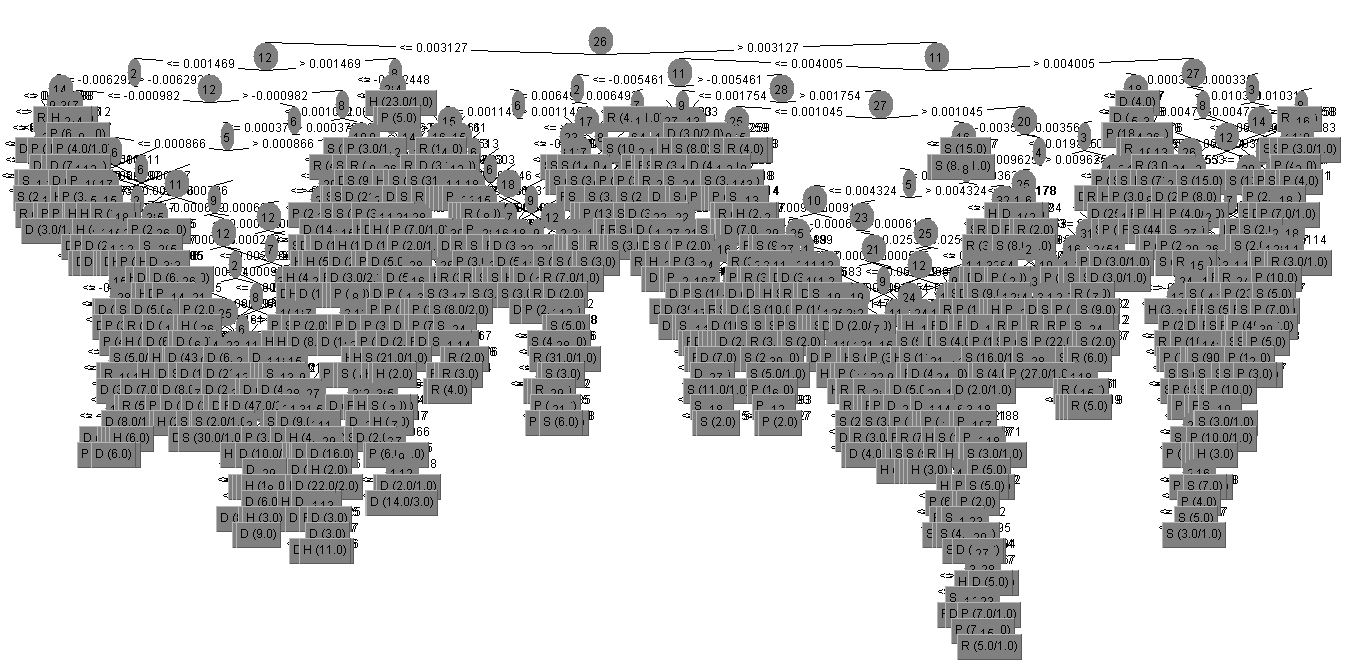
\includegraphics[width=0.95\textwidth]{05-j48}
	\caption{Árbol resultante del algoritmo J-48.}
	\label{fig:j48}
\end{figure}

El siguiente árbol utilizado para los experimentos fue creado usando el algoritmo LMT~\cite{Landwehr2005}.
Este árbol presentó un 98.26\% de eficiencia de aprendizaje tras entrenarse con el 60\% del dataset, probándose sobre las mismas instancias.
Una vez más, la eficiencia bajó sobremanera al probar con el 40\% restante, en el conjunto de pruebas:
53.10\% de los ejemplos bien clasificados.
El árbol resultante se presenta en la Figura~\ref{fig:lmt}, extraída directamente de WEKA.

\begin{figure}[htbp]
	\centering
	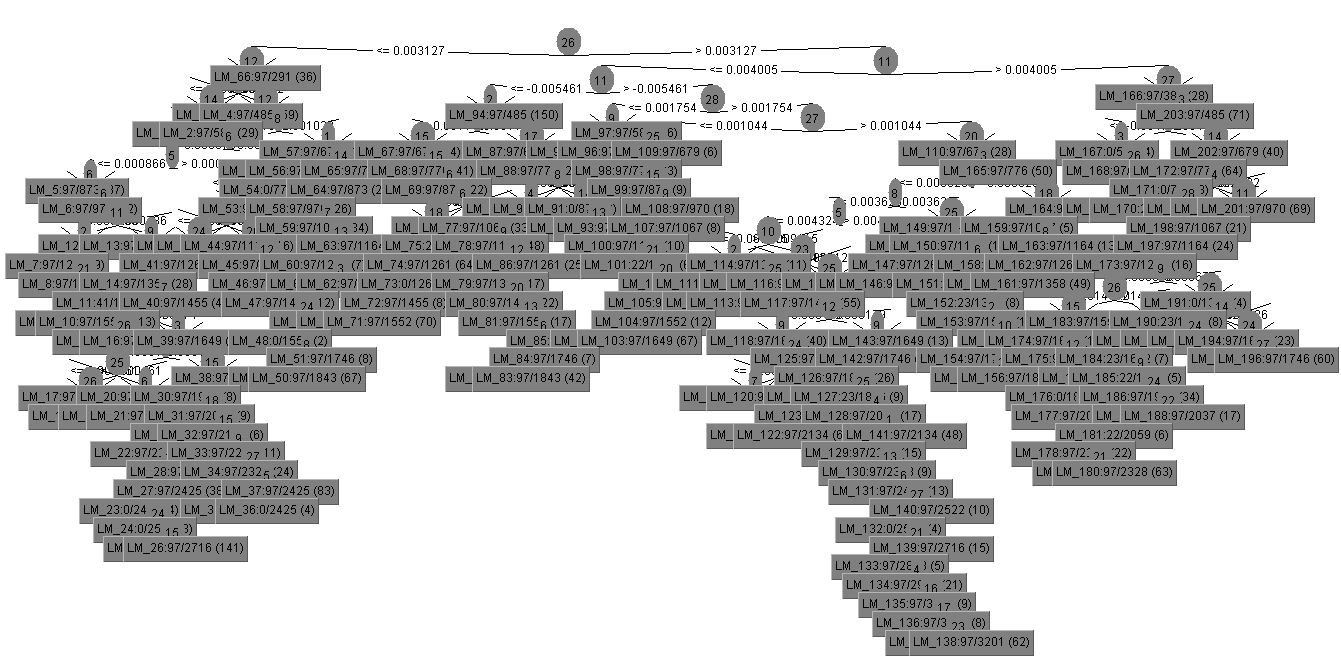
\includegraphics[width=0.95\textwidth]{05-lmt}
	\caption{Árbol resultante del algoritmo \textit{Logistic Model Tree} (LMT).}
	\label{fig:lmt}
\end{figure}

La tercer prueba fue realizada utilizando varios árboles aleatorios, técnica conocida como \textit{Random Forest}.
Las pruebas sobre el conjunto de entrenamiento fueron perfectas,
pues se logró clasificar correctamente el 100\% de los ejemplos (5924 instancias).
La eficiencia sobre el conjunto de pruebas, a pesar de haber disminuido,
se vio menos afectada que en los casos anteriores:
se alcanzó una eficiencia del 64.16\% sobre las 3949 instancias de prueba.

Tras llevar a cabo estos tres experimentos, se procedió a reducir el número de atributos del conjunto de datos para ver si había diferencia alguna con los árboles previamente generados.
Esta fase de preprocesamiento fue automática, utilizando el filtro \texttt{AttributeSelection} de WEKA.
Tras el nuevo tratamiento de datos (el cual redujo a 18 atributos el \textit{dataset}),
se procedió a partir en dos archivos: 60\% para entrenamiento y 40\% para pruebas, nuevamente.
Dos experimentos más se llevaron a cabo, una usando el algoritmo J48 y otra el LMT.

El árbol generado con J48 para el nuevo conjunto de entrenamiento (y probado sobre sí mismo)
logró un 90.73\% de ejemplos bien clasificados; cerca del 2\% menos que su versión sin selección de atributos.
Su eficiencia en el conjunto de prueba ascendió al 51.83\%, poco más del 1 porciento.
Por su parte, el porcentaje de eficiencia para el árbol generado con LMT sobre el conjunto de entrenamiento (y probado sobre sí mismo)
fue de 68.18\%; alrededor de 30\% menos que su versión sin selección de atributos.
Su eficiencia con el nuevo conjunto de pruebas se redujo cerca del 2\%,
pues alcanzó el 51.30\% de los ejemplos bien clasificados.

\subsection{Agrupamiento jerárquico}
\label{subsec:cluster}

Usando las mismas bases de datos para entrenamiento y pruebas (60\% y 40\% respectivamente),
se generaron modelos jerárquicos de agrupamiento utilizando WEKA.

El primer modelo, el cual fue generado sobre el conjunto de prueba (3949 instancias), separó en cinco grupos de la siguiente manera:
Grupo 1 de 1934 instancias (49\%), grupo 2 de 396 instancias (10\%),
grupo 3 de 1186 instancias (30\%), grupo 4 de 432 instancias (11\%)
y grupo 5 de una sola instancia.
Cabe mencionar que este modelo fue obtenido usando el método de algomeración de \textit{single link} y distancia euclidiana.

El segundo modelo que se intentó aplicar fue con las mismas características (\textit{single link} y distancia euclidiana)
pero sobre el conjunto de datos de entrenamiento (60\% de los ejemplos).
Sin embargo, este modelo no pudo completarse, incluso después de haber estado WEKA ejecución cerca de 11 horas.
Por lo mismo, decidió hacer un muestreo para contar con una base de ejemplos más pequeña, con 30\% de los mismos (2962 ejemplos).

Para una mejor comparación entre los nuevos modelos utilizados,
se presentan en la Figura~\ref{fig:classfreq} las frecuencias de las clases en el \textit{dataset}.

\begin{figure}[htbp]
	\centering
	\includegraphics[width=0.95\textwidth]{classfreq}
	\caption{Frecuencia de las clases en el conjunto de datos.
	De izquierda a derecha: $D, P, S, H, R$.}
	\label{fig:classfreq}
\end{figure}

Cada modelos probado fue etiquetado con distintos parámetros, los cuales son el tipo de vínculo entre los clústeres,
la métrica para distancia utilizada y si hubo selección de atributos o no.
La lista de operadores completa es la siguiente:

\begin{itemize}
	\item \texttt{A} para denotar que la base utilizada fue preprocesada por el filtro \texttt{AttributeSelection} de WEKA.
	\item \texttt{S} para referirse a los modelos hechos con el método \textit{single link}
	\item \texttt{C} para referirse a los modelos de hechos con el método \textit{complete-linkage}.
	\item \texttt{E} para etiquetar modelos con distancia euclideana.
	\item \texttt{M} para etiquetar modelos con distancia Manhattan.
\end{itemize}

Los porcentajes de cada grupo por modelo pueden ser observados en la Tabla~\ref{tab:cluster}.

\begin{table}[htbp]
\centering
\caption{Porcentaje de ejemplos por grupo, por modelo.}
\label{tab:cluster}
\begin{tabular}{@{}cccccc@{}}
\toprule
       & Grupo 1 & Grupo 2 & Grupo 3 & Grupo 4 & Grupo 5 \\ \midrule
Óptimo & 28      & 21      & 30      & 10      & 11      \\
\texttt{SE}     & 100     & 0       & 0       & 0       & 0       \\
\texttt{CE}     & 79      & 21      & 0       & 0       & 0       \\
\texttt{CM}     & 71      & 21      & 7       & 0       & 0       \\
\texttt{ASE}    & 11      & 49      & 30      & 10      & 0       \\
\texttt{ACE}    & 11      & 59      & 30      & 1       & 0       \\
\texttt{ASM}    & 100     & 0       & 0       & 0       & 0       \\
\texttt{ACM}    & 10      & 60      & 27      & 3       & 0       \\ \bottomrule
\end{tabular}
\end{table}

Como puede apreciarse en la Tabla~\ref{tab:cluster}, el proceso inverso a la clasificación supervisada varía mucho al utilizar los distintos parámetros disponibles de los algoritmos.

El modelo más cercano al óptimo fue el \texttt{ASE}: con selección de atributos, usando \textit{single-link clustering} y con distancia euclidiana.
Sin embargo, a pesar de ser el más cercano al óptimo, no es muy eficiente para clasificación.

La métrica euclidiana para la distancia parece obtener mejores resultados que la distancia Manhattan en este conjunto de datos.
Además, se puede notar que muchos modelos encontraron el óptimo del grupo 3, incluso cambiando el tipo de jerarquización.
Esto significa que el grupo 3 es más fácilmente identificable que los demás.

El grupo 2 fue bien clasificado en dos modelos,
los cuales utilizan vinculación completa para la jerarquización pero métricas distintas para medir la distancia.

\section{Conclusiones y Reflexiones}
\label{sec:conc}

Este trabajo revisó una serie de experimentos de clasificación y agrupamiento utilizando WEKA y un conjunto de datos de la literatura.

A pesar de tener una buena cantidad de datos (cerca de 10,000),
los resultados fueron muy variados dependiendo de los modelos utilizados.
Esto se puede deber a varias razones, pero sin duda una de ellas es la calidad de los datos.
Al tener una gran cantidad de atributos, es difícil establecer relaciones de proximidad entre los ejemplos.
Además, el hecho de que todos los atributos sean numéricos agrega una capa de abstracción adicional al conjunto de datos.

Asimismo, el tener resultados tan variados refleja la sensibilidad de la selección de modelos y sus distintos parámetros.
El ejercicio ha permitido interactuar de cerca con problemas comunes en el área de aprendizaje automático
y además conocer herramientas de la literatura que son frecuentemente utilizadas para problemas reales.

\bibliographystyle{splncs03}
\bibliography{05-biblio}

\end{document}